\subsubsection{Mathematical and Theoretical Physics}
\index{Schupp, Peter}

\paragraph{Research Team}
Peter Schupp (Professor), Robert Helling (Research Associate),
Sergey Solodukhin (Senior Research Associate), Wolfgang Spitzer
(Research Associate), Christian Blohmann  (Postdoctoral Fellow,
currently on leave to UC Berkeley),
 Matteo Rulli (PhD Student), %(has left IUB for industry in 2006)
  Jiangyang You (PhD Student)\\

Research Field: Modern mathematical physics; noncommutative field
theory, classical and quantum gravity, string theory, coherent
states, quantum spin systems.

General relativity is the basis of our understanding of stars,
galaxies and cosmology. It is a geometric theory of gravity: matter
curves space-time and particles propagate in this curved space.
Quantum physics on the other hand governs particles, atoms and
solids. Close to the Planck scale, where both gravitational and
quantum mechanical effects are equally important, we have to give up
the classical geometric idea of a smooth space-time manifold. To
model these quantum effects we have developed a noncommutative
gravity theory and are currently studying its exact solutions. The
mathematics that is used and advanced in this research is also
useful in other areas: We have been studying quantum spins in
ferromagnets, have developed tools for the analysis of the
anisotropy of the cosmic microwave background, and are currently
investigating applications in chemistry.

\paragraph{Highlights}

\null {\sl Non-commutative Gravity:} We have continued the
development of a quantum version of Einstein's theory of general
relativity in a way that preserves invariance under general
coordinate transformation \cite{Aschieri:2005yw}. This theory has
already had quite an impact. We have found Schwarzschild black hole
type solutions of the noncommutative gravity equations and have
discovered new principles underlying the theory. The theoretical
framework is still incomplete -- it does not completely fix the
non-commutative structure. We are using the quantized black hole
solutions as a theoretical laboratory to further our understanding
of the underlying physics.

\null {\sl Entanglement Entropy:} If one restricts the measurement
of quantum fields to lie outside of a given compact region, one
typically finds mixed states with respect to the restricted
observables -- even if the underlying state is pure globally. The
entropy arising this way is called ``entanglement entropy''. In many
situations it scales like the surface of the restricted region and
it is therefore thought of as toy model for the Beckenstein entropy
of black holes. In this context, we have studied the entanglement
entropy of black holes and Ricci flows
\cite{Solodukhin:2006ic,Solodukhin:2006xv}. The latter work extends
the irreversibility proof associated to the renormalization group
flow of 2d sigma models to higher dimensions. For the entanglement
entropy of non-relativistic fermions in one dimension, it has been
shown that the leading scaling includes a logarithm of the size. We
have generalized this result to higher dimensions and a large class
of geometries. This analysis involves asymptotic Fourier analysis
originally developed in information processing and has applications
to quantum gravity and convergence of the renormalization group
analysis of lattice systems.

\null {\sl Loop Quantum Gravity.} We continued our investigation of
quantization procedures employed in quantum gravity,  focusing on
covariance and continuity of the GNS states. By computing absorption
rates we have shown that in experimentally well studied systems the
``polymer representation'' used in the loop approach to quantum
gravity leads to unphysical absorption spectra
\cite{Helling:2006yn}.


\null {\sl Coherent States Analysis of the Cosmic Microwave
Background:}

The recent three-year cosmic microwave background (CMB) data from
the WMAP satellite can tell us a lot about cosmology and the
constituents of the universe: For instant, only a few percent of
matter is of the usual atomic type. The rest is dark matter and dark
energy, which we know very little about. It is believed that the CMB
is completely isotropic, i.e., independent of the region of the sky
that we look at. Looking at the large scale structure of the CMB
data, several research groups had however found some strange
alignment with a plane perpendicular to the ecliptic. We have
developed a very efficient way to analyse the CMB data using
coherent states. Our work confirms a surprising large-scale
anisotropy in the WMAP data and in addition shows that it persists
at smaller scales. We were able to show that it is not the ecliptic
that is relevant but the dipole direction, see
figure~\ref{fig:schupp}. We also found evidence that the anisotropy
is probably not of cosmic origin, but rather an artefact of the way
the WMAP data is analysed. We are currently analysing the CMB at
smaller scales and also seem to find structures that do not look as
random as expected \cite{Helling:2006xh}.
\begin{figure}[ht]
  \begin{center}
    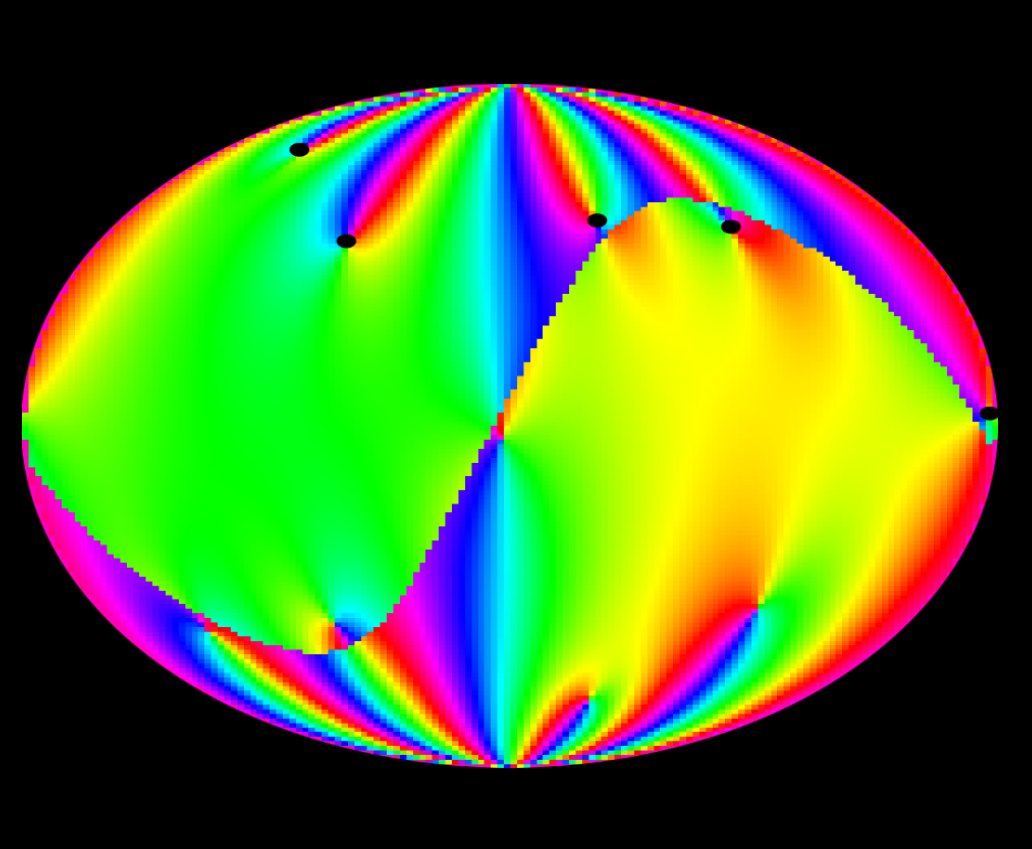
\includegraphics[width=6cm]{Schupp/schupp-fig.png}
    \mycaption{The cosmic microwave background analysed at $l=5$ has three of five multipole vectors aligned with the plane perpendicular to the dipole.
    }\label{fig:schupp}
   \end{center}
\end{figure}


\null {\sl Noncommutative Geometry as Quantization:} The transition
from pathological geometries to noncommutative spacetime algebras
was investigated as a quantization problem. Examples are the
irrational foliation of a 2-torus which quantizes to the
noncommutative torus algebra and the integration of the Dirac
structure of a magnetic monopole by a topological groupoid. A
mystery of the noncommutative torus algebra is that it does not
possess a Hopf structure, even though it is the quantization of a
group. We have resolved this by describing the pathological geometry
by a differentiable stack with a stacky Lie group structure, which
quantizes to a Morita invariant generalization of a Hopf structure,
called hopfish structure. The hopfish structure still yields a
tensor product of representations, which is needed for the
construction of the Fock space of a noncommutative quantum field
theory \cite{Blohmann:2006uj}.



\paragraph{Organization}
% list the (research) events you have organized, if any,

\begin{enumerate}
\item  Member of the Hochschulauswahlausschusses of German National
Scholarship Foundation (Studienstiftung)
\item International Center for Transdisciplinary Studies (ICTS),
scientific coordination (with B.\ Kramer and H.\ Meyer-Ortmanns)
\end{enumerate}

\paragraph{Collaborations}
\begin{enumerate}
\item {\sl Universit\"{a}t M\"{u}nchen and DESY Hamburg}\\
Prof. J. Wess\\
Noncommutative Gravity, Twisted General Relativity
\item {\sl Universit\"{a}t M\"{u}nchen}\\
Dr. B. Jurco\\
String Theory, Mathematics and Geometry of Stacks of D-branes
\item {\sl University of Zagreb, Croatia} \\
Prof. J. Trampetic \\
Noncommutative Standard Model and its Particle Physics
Phenomenology, Neutrino Dipole Moments
\item {\sl University of Vienna, Austria} \\
Prof. H. Grosse \\
Noncommutative Field Theory
\end{enumerate}


\paragraph{Grants}
% list the running grants in 2005, if none have been received, please delete this
% subsection.
\begin{enumerate}
\item Funded by DFG, \emph{Noncommutative Gravity}, \item Funded
by DFG, \emph{Nonabelian structures on D-branes and M-branes} DFG
Schwerpunktprogramm SSP 1096 ``Stringtheorie'',   \item Funded by
EU HRM OIF OIF-CT-2005-8559, \emph{Noncommutative Geometry} 
\end{enumerate}


\nocite{Schupp:2006ry,Solodukhin:2005ns,Solodukhin:2005ah,Bachmaier:2005jw}
